\section{Grad-CAM}
Grad-CAM is a white box method. The main parameter for this method is which layer that should be analyzed.

There are many existing implementations for this method, some of them using the PyTorch library.

TODO: how does it work?


\begin{figure}[h]
\centering
\caption{Image from original paper explaining some classes}
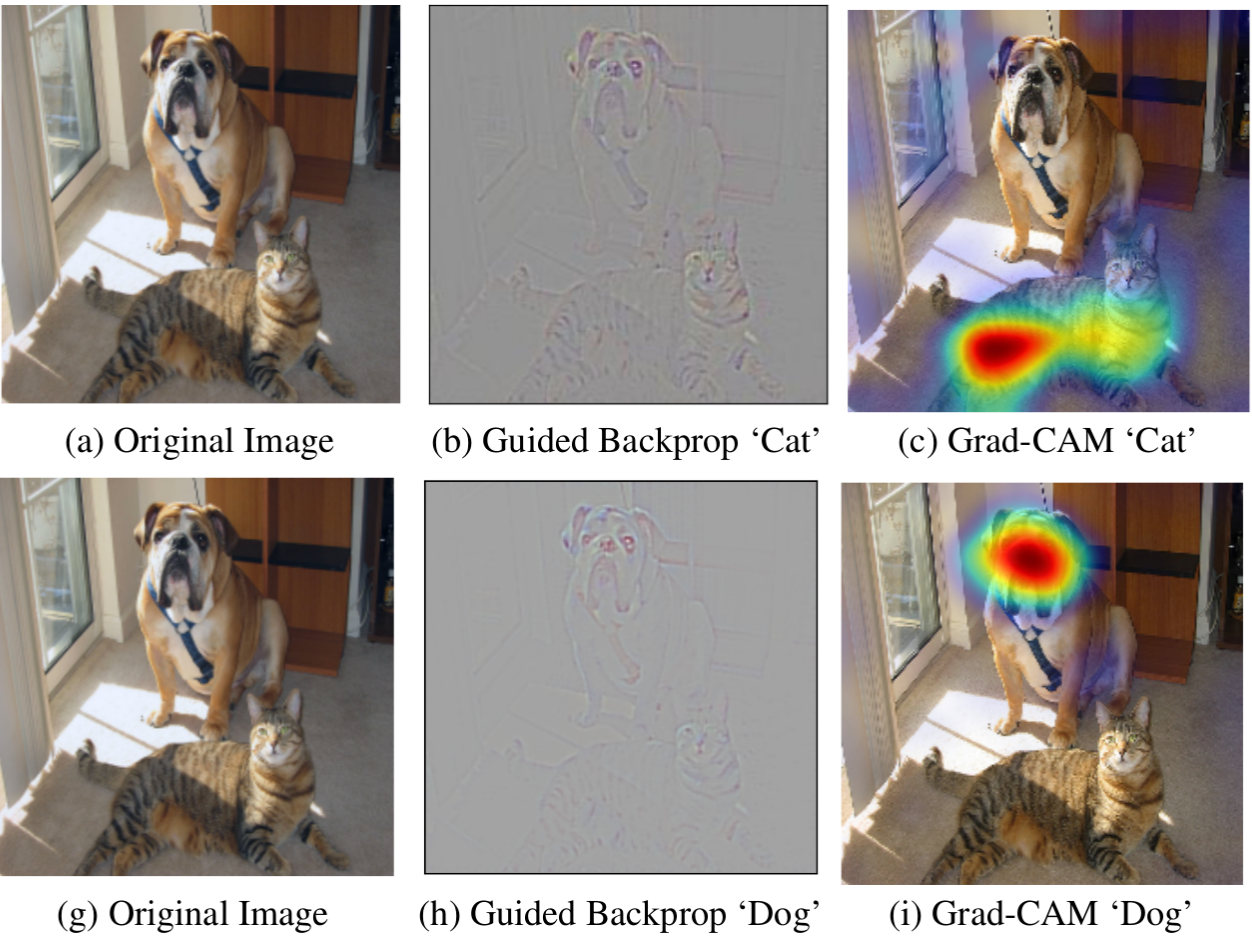
\includegraphics[width=14cm]{chapters/02_methods/images/grad-cam-example.png}
\end{figure}

\begin{figure}[h]
\centering
\caption{Grad-CAM explanation}
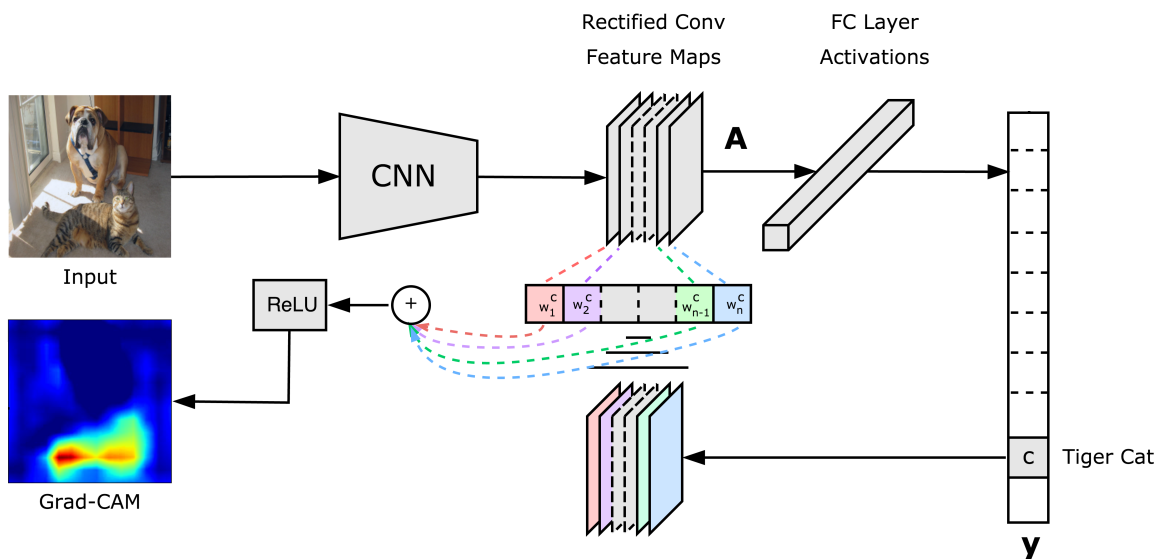
\includegraphics[width=14cm]{chapters/02_methods/images/grad-cam.png}
\end{figure}
